\documentclass[10pt]{article}
\usepackage{tikz}
\usetikzlibrary{shapes.misc}
\usepackage[margin=0cm]{geometry}
\pagestyle{empty}
\tikzstyle{every node}=[cross out, draw, red]

\begin{document}

\vspace*{\fill}
\begin{center}
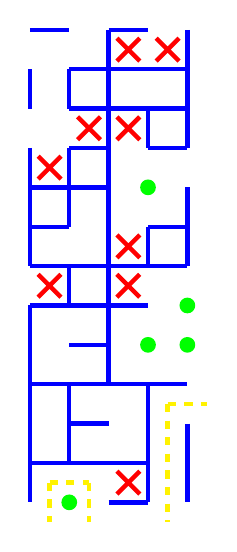
\begin{tikzpicture}[x=0.5cm, y=-0.5cm, ultra thick, blue]
% Walls
    \draw (0,0) -- (1,0);
    \draw (2,0) -- (3,0);
    \draw (1,1) -- (4,1);
    \draw (1,2) -- (4,2);
    \draw (1,3) -- (2,3);
    \draw (3,3) -- (4,3);
    \draw (0,4) -- (2,4);
    \draw (0,5) -- (1,5);
    \draw (3,5) -- (4,5);
    \draw (0,6) -- (4,6);
    \draw (0,7) -- (3,7);
    \draw (1,8) -- (2,8);
    \draw (0,9) -- (4,9);
    \draw (1,10) -- (2,10);
    \draw (0,11) -- (3,11);
    \draw (2,12) -- (3,12);
    \draw (0,1) -- (0,2);
    \draw (0,3) -- (0,6);
    \draw (0,7) -- (0,12);
    \draw (1,1) -- (1,2);
    \draw (1,3) -- (1,5);
    \draw (1,6) -- (1,7);
    \draw (1,9) -- (1,11);
    \draw (2,0) -- (2,9);
    \draw (3,2) -- (3,3);
    \draw (3,5) -- (3,6);
    \draw (3,9) -- (3,12);
    \draw (4,0) -- (4,3);
    \draw (4,4) -- (4,6);
    \draw (4,10) -- (4,12);
% Pillars
    \fill[green] (3,4) circle(0.2);
    \fill[green] (4,7) circle(0.2);
    \fill[green] (3,8) circle(0.2);
    \fill[green] (4,8) circle(0.2);
    \fill[green] (1,12) circle(0.2);
% Inner points in accessible cul-de-sacs
    \node at (2.5,0.5) {};
    \node at (3.5,0.5) {};
    \node at (1.5,2.5) {};
    \node at (2.5,2.5) {};
    \node at (0.5,3.5) {};
    \node at (2.5,5.5) {};
    \node at (0.5,6.5) {};
    \node at (2.5,6.5) {};
    \node at (2.5,11.5) {};
% Entry-exit paths without intersections
    \draw[dashed, yellow] (3.5,9.5) -- (4.5,9.5);
    \draw[dashed, yellow] (0.5,11.5) -- (1.5,11.5);
    \draw[dashed, yellow] (0.5,11.5) -- (0.5,12.5);
    \draw[dashed, yellow] (1.5,11.5) -- (1.5,12.5);
    \draw[dashed, yellow] (3.5,9.5) -- (3.5,12.5);
\end{tikzpicture}
\end{center}
\vspace*{\fill}

\end{document}
